\documentclass[a4paper,10pt,twoside]{article}
%%%%%%%%%%% Packages %%%%%%%%%%
\usepackage[margin=1in]{geometry}
\usepackage{amsmath, amssymb,mathtools}
\usepackage{fancyhdr}
\usepackage{sectsty}
\usepackage{graphicx,wrapfig}
\usepackage{enumitem}
\usepackage{float}
\usepackage{braket}
\usepackage{bbm}
\usepackage{tikz,calc}

%%%%%%%%%%% Macros %%%%%%%%%%
\def \note#1 {\vspace{-1em}\paragraph{\bfseries #1}}
\def \dd {{\rm d}}
\def \id {{\mathbbm{1}}}
\def \order {\mathcal{O}}
\def\bquad{\mkern-18mu}
\DeclareMathOperator{\trace}{tr}
\DeclareMathOperator{\spanset}{span}

%%%%%%%%%%% Tikz Definitions %%%%%%%%%%
\usetikzlibrary{shapes, arrows,positioning,fit,automata}
\tikzstyle{plain} = [draw,thick,circle,inner sep=0,minimum size=0.5cm,font=\footnotesize]
\tikzstyle{mps} = [draw,thick,rectangle,rounded corners=.1cm,inner sep=0,minimum size=0.5cm]
\tikzstyle{mpo} = [draw,thick,circle,inner sep=0,minimum size=0.5cm]
\tikzstyle{index} = [-,thick,font=\footnotesize]
\tikzstyle{virtual} = [-,thick,dotted,font=\footnotesize]
\tikzstyle{site} = [draw,solid,circle,minimum size=2pt,inner sep=0pt,outer sep=0pt,fill=black]

\def \tu {0.25cm}

%%%%%%%%%%% Formatting %%%%%%%%%%
\pagestyle{fancy}
\renewcommand{\footrulewidth}{0.5pt}

\fancyhf{}
\lhead{22/07/2017}
\chead{Quantum Information Methods in Many-Body Physics}
\rhead{PH2269}
\lfoot{Giacomo Giudice~~~~giacomo.giudice@mpq.mpg.de}
\rfoot{Page \thepage}

\allsectionsfont{\normalfont\sffamily}

%%%%%%%%%%% Here Begins Document %%%%%%%%%%
\begin{document}
\title{\vspace{-1cm}\sffamily Homework 7\vspace{-1cm}}
\author{}
\date{}
\maketitle
\thispagestyle{fancy}

\begin{section}{MPO and Finite State Automata}
\paragraph{Introduction} Recall the tensor network representation of a \emph{Matrix Product Operator} (MPO).
We are particularly interested in representing an  Hamiltonian of an $N$-body one-dimensional system
\[
  H =
  {
  \tikz[baseline=-0.5*\tu,node distance=\tu]{
      \node[mpo]  (mpo1) {};
      \draw[index] (mpo1.north) -- +(0,\tu);
      \draw[index] (mpo1.south) -- +(0,-\tu);
      \def\lastn{1}
      \foreach \n[remember=\n as \lastn] in {2,...,8} {
        \node[mpo,right=of mpo\lastn]  (mpo\n) {};
        \draw[index] (mpo\n.west) -- (mpo\lastn.east);
        \draw[index] (mpo\n.north) -- +(0,\tu);
        \draw[index] (mpo\n.south) -- +(0,-\tu);
      }
    }
  }\ .
\]
For concreteness, let us start by considering the following Hamiltonian
\[
  H = \sum_{i=1}^N X_i, \quad X_i = \underbrace{\id \otimes \dots \otimes \id}_{(i-1) \mbox{~times}} X \underbrace{\id \otimes \dots \otimes \id}_{(N-i) \mbox{~times}} ,
\]
where $X$ is some local operator on site $i$. 
By labeling the local operators with states (or characters) from a finite alphabet $\Sigma = \{\texttt{0},\texttt{1}\}$, $\id \sim \texttt{0}$, $X \sim \texttt{1}$, we can rewrite the Hamiltonian as a series of strings,
\[
  H \sim \texttt{10000\dots} +  \texttt{01000\dots} +  \texttt{00100\dots} +  \texttt{00010\dots} + \dots
\]
We can then view the MPO associated to $H$ as a \emph{Finite State Automaton}, that goes through a string $a_1 \dots a_N$, $a_i \in \Sigma$, accepting it or rejecting it.
The MPO is then a machine that just takes a string, and checks if it matches some kind of pattern. 
If it matches, it outputs a weight $W$ corresponding to the correct pre-factor for each term in the Hamiltonian.
Otherwise, the pattern is rejected.
The resulting Hamiltonian is then the sum of all possible combinations of valid inputs.

In this finite automata picture, each tensor in the chain takes an input states $l,r \in Q$, on the virtual level, and produces outputs state $a \in \Sigma$ on the physical level.
Since neighboring tensors share a virtual leg, the inputs on the shared legs must be equal.

\[
  {
  \tikz[baseline=-0.5*\tu,node distance=\tu]{
      \node[mps]  (m) {};
      \draw[index,->] (m.north) -- +(0,\tu) node[above]{$a$};
      \draw[index,<-] (m.west) -- +(-\tu,0) node[left]{$l$};
      \draw[index,<-] (m.east) -- +(\tu,0) node[right]{$r$};
    }
  }
\]

The way a tensor produces its output is called a \emph{rule}. 
Convince yourself that the rules for the previous Hamiltonian are
\[
  \left\{
  {
  \tikz[baseline=-0.5*\tu,node distance=\tu]{
      \node[mps]  (m) {};
      \draw[index] (m.north) -- +(0,\tu) node[above]{$\texttt{0}$};
      \draw[index] (m.west) -- +(-\tu,0) node[left]{0};
      \draw[index] (m.east) -- +(\tu,0) node[right]{0};
    }
  },
  {
  \tikz[baseline=-0.5*\tu,node distance=\tu]{
      \node[mps]  (m) {};
      \draw[index] (m.north) -- +(0,\tu) node[above]{$\texttt{1}$};
      \draw[index] (m.west) -- +(-\tu,0) node[left]{0};
      \draw[index] (m.east) -- +(\tu,0) node[right]{1};
    }
  },
  {
  \tikz[baseline=-0.5*\tu,node distance=\tu]{
      \node[mps]  (m) {};
      \draw[index] (m.north) -- +(0,\tu) node[above]{$\texttt{0}$};
      \draw[index] (m.west) -- +(-\tu,0) node[left]{1};
      \draw[index] (m.east) -- +(\tu,0) node[right]{1};
    }
  }
  \right\}
\]
Equivalently, we can think of the automaton as a walker having an internal state. 
At each site it outputs a state $a$  and can change its internal state according to the set of rules.
As in the example above, the transitions may not be unique.
We can then represent the finite automaton by a transition map
\begin{figure}[H]
  \centerline{
  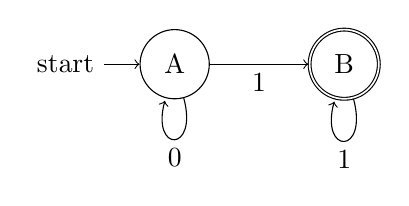
\begin{tikzpicture}[auto,node distance=5*\tu]
    \node[initial,state] (A) {A};
    \node[state,accepting,right=of A] (B) {B};
    \path[->] (A) edge[left] node[below]  {1} (B);
    \path[->] (A) edge[loop below] node[below]  {0} (A);
    \path[->] (B) edge[loop below] node[below]  {1} (B);
  \end{tikzpicture}
  }
\end{figure}
where the highlighted node indicates the input of the automation is ``accepting''.
In this case the weight of the accepting state is set to 1.

The corresponding tensor $M$ of the MPO is straightforward to write, we put the different states into a matrix generated by the column index $l$ and the row index $r$
\[
  M = 
  \begin{pmatrix}
  \id & X \\
  0 & \id
  \end{pmatrix} ,
\]
in which each entry of the matrix acts on the physical indices of the tensor.
Explicitly perform the matrix multiplication to show that the tensor $M$ generates the original Hamiltonian.
What are the tensors at the boundary (assuming open boundary conditions)?

\paragraph{Nearest-Neighbor Interaction}  Using the same character labels, compute the rules, the transition diagram and the MPO tensor for the Hamiltonian
\[
  H \sim  \texttt{11000\dots} +  \texttt{01100\dots} +  \texttt{00110\dots} +  \texttt{00011\dots} + \dots
\]
Notice how this Hamiltonian couples nearest-neighbors.

\paragraph{Heisenberg Model} Generalize the previous result to compute the MPO for the celebrated Heisenberg Hamiltonian for spin-1/2 particles,
\[
  H = \sum_{i=1}^{N-1} \vec{S}_i \cdot \vec{S}_{i+1} .
\]
\paragraph{Next Nearest-Neighbor Interaction} Find the MPO representation of the Hamiltonian
\[
  H =  J_1 \sum_i Z_i Z_{i+1} + J_2 \sum_i Z_i Z_{i+2} .
\]

\paragraph{Long-Range Interactions} Show that the tensor
\[
  M = 
  \begin{pmatrix}
  \id & X & 0 \\
  0 & \lambda \id & J \lambda X \\
  0 & 0 & \id
  \end{pmatrix} ,
\]
gives rise to exponentially decaying interaction 
\[
  H = \sum_{i=1}^N \sum_{r>0} J e^{-r/\xi} X_i X_{i+r} .
\]
As a closing remark, we can approximate any arbitrary interaction $J(r)$ as a sum of exponentially decaying interactions\footnote{G.M. Crosswhite, A.C. Doherty, G. Vidal, Phys. Rev. B (2008) arXiv:0804.2504 and 
F. Fr{\"o}wis, V. Nebendahl, W. D{\"u}r, Phys. Rev. A (2010) arXiv:1003.1047}, simply by finding the scalars $c_\alpha$ that minimize the distance $ \| J(r) - \sum_\alpha \lambda_\alpha^r \|^2$.


\note{Note} Notice how the bond dimension $\chi$ corresponds and the number of states $|Q|$ of the finite automaton.
\end{section}

\begin{section}{MPS Expectation Values*}
Construct the MPS representation for the states $\ket{\uparrow \uparrow \dots \uparrow \uparrow}$, $\ket{\downarrow \downarrow \dots \downarrow \downarrow}$ and $\ket{\rm GHZ}$ for 10-50 sites.
Create a function to numerically compute overlaps between MPS and calculate the overlaps between the previous states.
Now construct the MPO for the Heisenberg model $H = \sum_i \vec{S}_i \cdot \vec{S}_{i+1}$ and compute the expectation values $\braket{H}$ for the states above.

\note{Tips} If you don't have experience with handling tensors, let me break it down into smaller steps
\begin{enumerate}[label=(\alph*)]
  \item Use some package\footnote{For  Matlab/Octave I recommend \texttt{ncon}, available in the supplementary material of arXiv:1402.0939. Multiple options exist for Python, but you may start off with \texttt{tensordot} or \texttt{einsum}. For Julia, try the \texttt{TensorOperations} package.}, to familiarize yourself with contracting tensors.
  \item Define an index order convention for your MPS and MPO tensors, such as \texttt{(left,right,up)}.
  \item Construct your MPS/MPO as an array of tensors, one for each site.
  \item When computing your overlap, mind the contraction order!
\end{enumerate}
\end{section}
\end{document}
%%%%%%%%%%% Here Ends Document %%%%%%%%%%
